\documentclass[../relazione.tex]{subfiles}
\graphicspath{{\subfix{../images/}}}

\begin{document}
\section{Terza implementazione}

Per la terza implementazione sono stati ordinati i task prima di passarli al \textit{compute\_metrics} kernel, in questo modo non è necessario controllare che il kernel non cambi la \textit{next\_queue} ma semplicemente deve essere lanciato un numero di volte pari al numero dei livelli.

In realtà questa cosa non ha senso, perché non ho un modo veloce per calcolare il livello di un nodo, dovrei fare qualcosa di molto simile al kernel compute metrics attuale e non avrebbe senso a quel punto non calcolare contestualmente anche il peso.

\subsection{Fase 1 - Ricerca degli entrypoint}
Grazie alla nuova struttura per verificare che un nodo sia un entrypoint è sufficiente controllare che la prima posizione della colonna relativa al nodo in esame abbia almeno un elemento, cosa che si traduce nel controllare che il primo elemento della colonna esista. 
\begin{lstlisting}[language=C++, caption={Find entrypoints kernel II},captionpos=b]
kernel void entry_discover_rectangular(const int n_nodes, global edge_t* restrict edges, volatile global int* n_entries, global int* entries)
{
	int current_node_index = get_global_id(0);
	if (current_node_index >= n_nodes) return;

	if (edges[matrixToArrayIndex] <= -1)
		entries[i] = 1;
}
\end{lstlisting}

\subsection{Fase 2 - Calcolo delle metriche}
La differenza rispetto alla prima implementazione risiede solo nel diverso accesso alla matrice di adiacenza.

\clearpage
\begin{lstlisting}[language=C++, caption={Compute metrics kernel II},captionpos=b]
kernel void compute_metrics_rectangular(global int* restrict nodes, global int* queue_, global int* next_queue_, const int n_nodes, global edge_t* restrict edges, global edge_t* restrict edges_reverse, volatile global int2* metriche, const int max_adj_dept)
{
	int current_node_index = get_global_id(0);
	if(current_node_index >= n_nodes) return;
	
	[...] //omissis of various security checks
	
	for (int j = 0; j < max_adj_dept; j++) {
		int parentAdjIndex = j;
		matrixToArrayIndex = matrix_to_array_indexes(parentAdjIndex, current_node_index, n_nodes);
		int edge_weight = 1;
		int parent_index = edges[matrixToArrayIndex];
		if (parent_index >= 0){
			int weight_with_this_parent = edge_weight + metriche[parent_index].x + nodes[current_node_index];
			int level_with_this_parent = metriche[parent_index].y + 1;
			metrics_with_this_parent = (int2)(weight_with_this_parent, level_with_this_parent);
			if (gt(metrics_with_this_parent, metriche[current_node_index]))
				metriche[current_node_index] = metrics_with_this_parent;
		}
		int child_index = edges_reverse[matrixToArrayIndex];
		if (child_index >= 0)
			atomic_inc(&next_queue_[child_index]);
	}
}
\end{lstlisting}

Anche in questo caso il kernel deve essere eseguito dall'host più volte fin quando non si produrrà una \textit{next\_queue} identica alla precedente in cui quindi non ci sono stati cambiamenti.

\subsection{Fase 3 - ordinamento dei task}
In questa fase non è stato modificato nulla in quanto si lavora su un array di metriche che non ha alcuno correlazione alla matrice di adiacenza e che quindi non è influenzata dalle modifiche a quest'ultima,

\subsection{Considerazioni}
La complessità di questa seconda implementazione è $O(n)$ per la ricerca degli entrypoint, $O(n \cdot max\_adj\_dept)$ per il calcolo delle metriche e $O(n\ log\ n)$.
In definitiva, l'algoritmo ha complessità $O(n \cdot max\_adj\_dept)$, dove $n$ è il numero di nodi e $max\_adj\_dept$ è il numero massimo di figli che un nodo può avere.

\subsection{Variazioni}
Anche in questo caso si è provato a vettorizzare il kernel per abbassare i tempi di runtime che, comunque, rispetto alla prima implementazione sono già più bassi di diversi ordini di grandezza.

Sarebbe stato inutile inoltre verificare eventuali variazioni con la matrice trasposta, in quanto già nell'implementazione base sfruttiamo due matrici di adiacenza, una che tiene traccia dei figli di ogni nodo ed una speculare che tiene traccia dei genitori.

Riportiamo di seguito i tempi di runtime dei kernel con la nuova implementazione e successivamente il confronto tra il \textit{compute\_metrics} più basso della prima implementazione e quello della seconda implementazione compresa la sua variante vettorizzata.

Anche in questo caso per i testi si è usato un dataset di 4096 task in esecuzione su una GPU NVIDIA GTX 1650 per 20 esecuzioni di cui successivamente è stata calcolata la media dei tempi di runtime.\\

\begin{figure}[h]
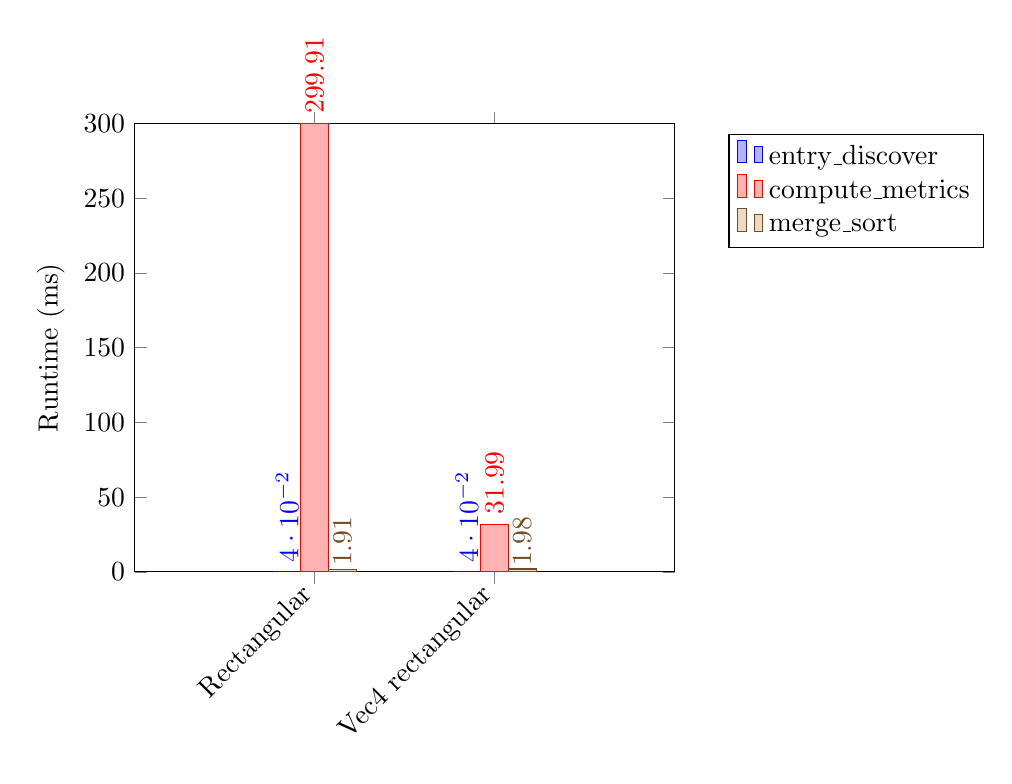
\begin{tikzpicture}
\begin{axis}[
symbolic x coords={
Rectangular,
Vec4 rectangular},
xtick=data,
x tick label style={rotate=45,anchor=east},
nodes near coords,
every node near coord/.append style={rotate=90, anchor=center},
ylabel=Runtime (ms),
legend style={at={(1.1, 0.85)}, anchor=west},
ybar=0pt,
legend cell align={left},
enlarge x limits=1,
enlarge y limits=0,
]
\addplot+[every node near coord/.append style={yshift=10pt, xshift=30pt}] coordinates { %entries discover
(Rectangular, 0.04)
(Vec4 rectangular, 0.04)
};
\addplot+[every node near coord/.append style={xshift=0pt, anchor=west}] coordinates { %compute metrics
(Rectangular, 299.91)
(Vec4 rectangular, 31.99)
};
\addplot+[every node near coord/.append style={yshift=-10pt, xshift=0pt}] coordinates { %mergesort
(Rectangular, 1.91)
(Vec4 rectangular, 1.98)
};
\legend{entry\_discover, compute\_metrics, merge\_sort}
\end{axis}
\end{tikzpicture}
\caption{Tempi di runtime della seconda implementazione}
\end{figure}

\\

\begin{figure}[h]
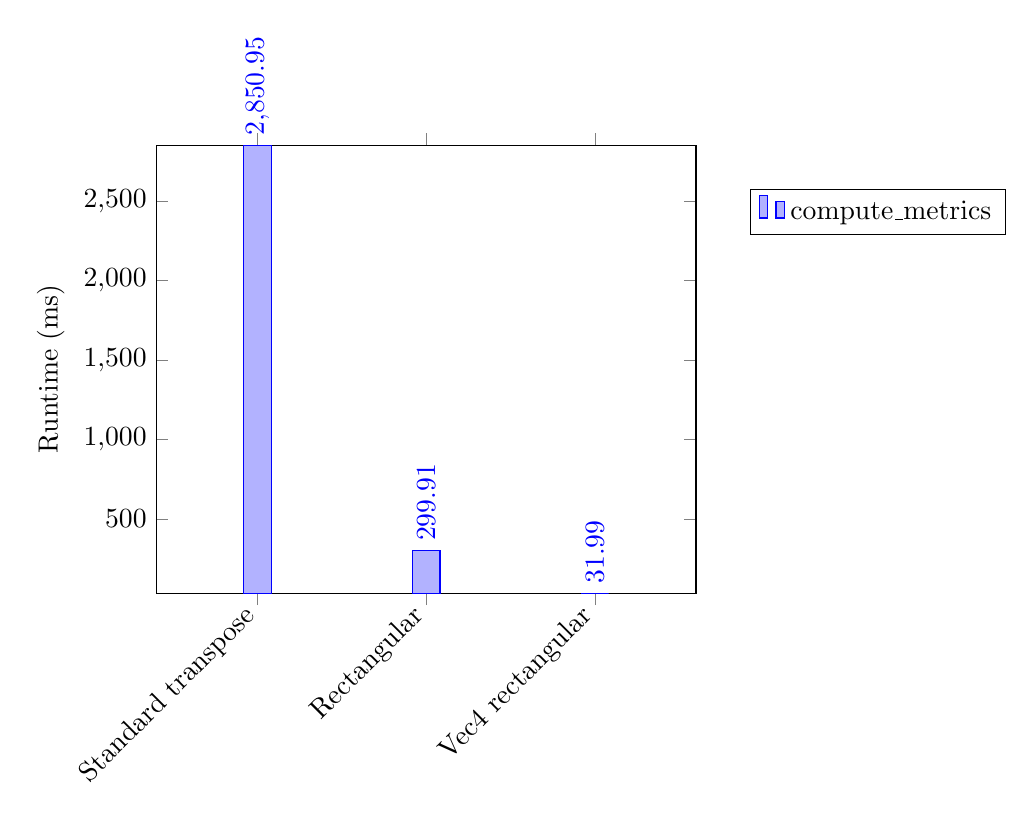
\begin{tikzpicture}
\begin{axis}[
symbolic x coords={
Standard transpose,
Rectangular,
Vec4 rectangular},
xtick=data,
x tick label style={rotate=45,anchor=east},
nodes near coords,
every node near coord/.append style={rotate=90, anchor=center},
ylabel=Runtime (ms),
legend style={at={(1.1, 0.85)}, anchor=west},
ybar=0pt,
legend cell align={left},
enlarge x limits=0.3,
enlarge y limits=0,
]
\addplot+[every node near coord/.append style={xshift=0pt, anchor=west}] coordinates { %compute metrics
(Standard transpose, 2850.95)
(Rectangular, 299.91)
(Vec4 rectangular, 31.99)
};
\legend{compute\_metrics}
\end{axis}
\end{tikzpicture}
\caption{Tempi di runtime della prima e della seconda implementazione a confronto} \label{fig:M1}
\end{figure}


Quindi come si può vedere non solo le prestazioni sono influenzate incredibilmente dalla velocità del kernel che calcola le metriche ma, inoltre, i tentativi di migliorare le prestazioni vettorizzando il kernel hanno solo peggiorato la situazione. 

\end{document}